\documentclass[border=10pt]{standalone}
\usepackage{xcolor}
\usepackage{pgfplots}
\usepackage{tikz}
\begin{document}
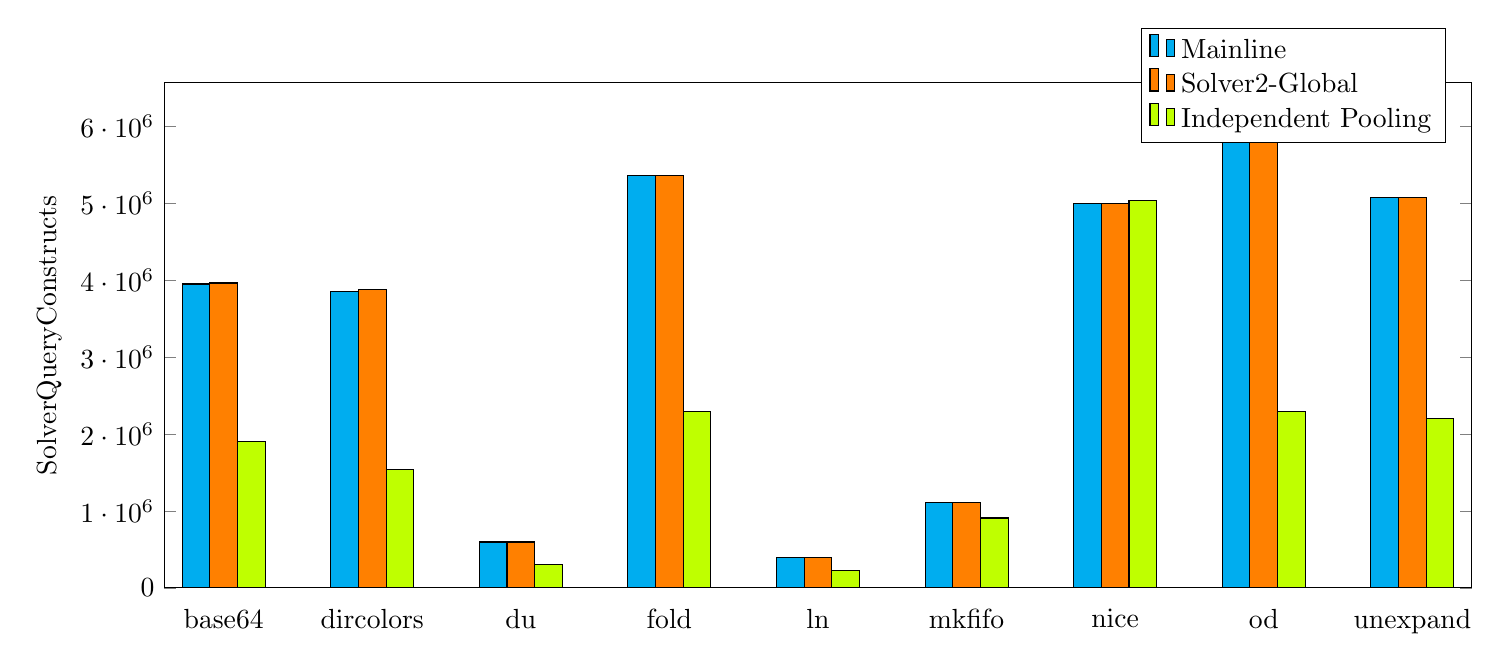
\begin{tikzpicture}
    \begin{axis}[
        width  = 1.5 * \textwidth,
        height = 8cm,
        major x tick style = transparent,
        % tickwidth=10,
        ybar=0,
        bar width=10pt,
        % ymajorgrids = true,
        ylabel = {SolverQueryConstructs},
        symbolic x coords={base64,dircolors,du,fold,ln,mkfifo,nice,od,unexpand},
        xtick = data,
        scaled y ticks = false,
        enlarge x limits=0.05,
        ymin=0,
        legend cell align=left,
        legend style={
                at={(0.98,0.88)},
                anchor=south east,
                % column sep=1ex
        }
    ]
        \addplot[style={cyan,fill=cyan,mark=none}, draw=black]
	coordinates {(base64,3952443) (dircolors,3860098) (du,596868) (fold,5362146) (ln,392868) (mkfifo,1110073) (nice,4996319) (od,5975818) (unexpand,5080470)};
\addplot[style={orange,fill=orange,mark=none}, draw=black]
	coordinates {(base64,3966386) (dircolors,3883287) (du,596868) (fold,5362146) (ln,392021) (mkfifo,1110075) (nice,4996319) (od,5975303) (unexpand,5080470)};
\addplot[style={lime,fill=lime,mark=none}, draw=black]
	coordinates {(base64,1898754) (dircolors,1542663) (du,299412) (fold,2290270) (ln,222237) (mkfifo,909366) (nice,5043510) (od,2299046) (unexpand,2205504)};

        \legend{Mainline,Solver2-Global,Independent Pooling}
    \end{axis}
\end{tikzpicture}
\end{document}
